\documentclass[12pt, a4paper]{article}

% Text languages
\usepackage[spanish, english, UKenglish, USenglish, american, british]{babel}

% Accents
\usepackage[latin1]{inputenc}

% Maths
\usepackage{mathtools}
\usepackage{amsmath}

\DeclarePairedDelimiter\abs{\lvert}{\rvert}%
\DeclarePairedDelimiter\norm{\lVert}{\rVert}%

% Swap the definition of \abs* and \norm*, so that \abs
% and \norm resizes the size of the brackets, and the 
% starred version does not.
\makeatletter
\let\oldabs\abs
\def\abs{\@ifstar{\oldabs}{\oldabs*}}
%
\let\oldnorm\norm
\def\norm{\@ifstar{\oldnorm}{\oldnorm*}}
\makeatother


% https://www.overleaf.com/learn/latex/Page_size_and_margins
\usepackage{geometry}
\topmargin = -23pt
\oddsidemargin = 13pt
\headheight = 12pt
\headsep = 25pt
\textheight = 674pt
\textwidth = 426pt
\marginparsep = 10pt
\marginparwidth = 50pt
\footskip = 30pt
\marginparpush = 5pt
\hoffset = 0pt
\voffset = 0pt
\paperwidth = 597pt
\paperheight = 845pt

% Hyperlinks
\usepackage{hyperref}

% Figure
\usepackage{graphicx}
% \usepackage{subcaption}

% Example
\newtheorem{exmp}{Example}[section]
%--------------------------------------------------------------------------
\title{Detection of/between similarity of documents with hashing}
\author{Roger Vilaseca Darn� and Xavier Mart�n Ballesteros\\
  \small Algorithms\\
}
\date{1st December 2018}

\begin{document}
% Images
\graphicspath{ {./images/} }

\maketitle
%\abstract{Esto es una plantilla simple para un articulo en \LaTeX.}


\section{Introduction}

% Refer�ncia a una equaci� \ref{eq:area}).
% Refer�ncia a una secci� \ref{sec:nada}
% Refer�ncia a una cita \cite{Cd94}.

\section{Jaccard Index}
The Jaccard Index, also known as Intersection Over Union (IOU), calculates the percentage of similarity between two sets.

For any pair of sets S and T, the Jaccard Index is defined as:
% For any pair of sets S and T, we can define the Jaccard Index as shown:
\begin{equation}
J(S, T) = \frac{\abs{S \cap T}}{\abs{S \cup T}}
\end{equation}

We can easily deduce that the more common words, the bigger the Jaccard Index, which means that it is more probable that one set is a duplicate of the other.

\begin{exmp}
In Figure \ref{fig:JaccardExample} we see two sets S and T. There are 3 elements in their intersection ("I", "love", "chocolate") and 6 in their union ("I", "love", "chocolate", "and", "pizza", "white"). Thus, J(S, T) = 3/6.

\begin{center}
	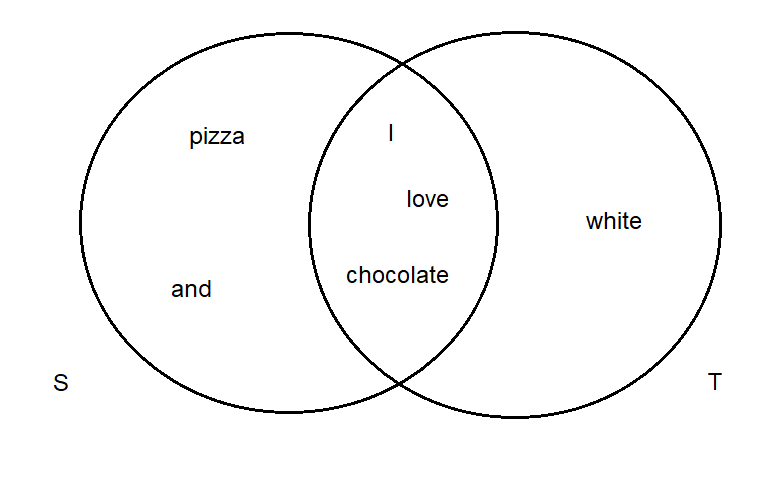
\includegraphics[width=3in]{JaccardExample}
	\label{fig:JaccardExample}
	
	Figure \ref{fig:JaccardExample}: Two sets with Jaccard Index 3/6.
\end{center}

% Falta dir qu� passa si hi ha poques paraules? Fals positiu...?

\end{exmp}

\section{Shingling of Documents}

Any pair of documents can be compared by watching the number of repeated strings they have.
\underline{The more common strings, the more probable is that one is a duplicate from the other.}
One way to represent a document as a set is to insert in the set each string that appears in it. If we do so, then duplicated documents that have reorganized the sentences or even the entire text will have plenty of common strings, and will be \underline{caught}.

\subsection{k-Shingles}

The idea is not to insert in the set all the words, but a set of characters of size \textit{k}. Thus, each element of the set will have the same size as the others.

The question now is how big \textit{k} should be? If we take a small value of \textit{k}, this will result in many shingles that are present in all documents. Suppose we choose the extreme case (\textit{k} = 1). Then, all documents would result to be similar, as the most used characters are present in all documents. However, if we take a big value of \textit{k}, then any pair of documents would not share a shingle.

The value of \textit{k} depends on the size of the documents. A poem will not have the same \textit{k} value than an article. Otherwise, we could have the problems mentioned before.
The important idea in order to choose a good \textit{k} is:
\emph{k should be picked large enough that the probability of any given shingle appearing in any given document is low.}

\section{Minhashing}

Mas texto.

\section{Locality Sensitive Hashing (LSH)}

Mas texto.

\subsection{Referencies}

\url{https://towardsdatascience.com/understanding-locality-sensitive-hashing-49f6d1f6134}


\url{https://santhoshhari.github.io/Locality-Sensitive-Hashing/}

\url{https://www.youtube.com/watch?v=96WOGPUgMfw}

\url{https://www.youtube.com/watch?v=_1D35bN95Go}

\url{https://medium.com/engineering-brainly/locality-sensitive-hashing-explained-304eb39291e4}

\url{http://www.mit.edu/~andoni/LSH/}

\url{http://infolab.stanford.edu/~ullman/mmds/ch3.pdf}


% Bibliograf�a.
%-----------------------------------------------------------------
\begin{thebibliography}{99}

\bibitem{Cd94} Author, \emph{Title}, Editor, (year)

\end{thebibliography}

\end{document}